\documentclass[12pt,a4paper]{article}
\usepackage[utf8]{inputenc}
\usepackage{fullpage}
\usepackage[top=2cm, bottom=4.5cm, left=2.5cm, right=2.5cm]{geometry}
\usepackage{amsmath,amsthm,amsfonts,amssymb,amscd}
\usepackage{lastpage}
\usepackage{enumerate}
\usepackage{fancyhdr}
\usepackage{mathrsfs}
\usepackage{xcolor}
\usepackage{graphicx}
\usepackage{listings}
\usepackage{hyperref}
\usepackage{setspace}
\usepackage{array} 
\usepackage{paralist} 
\usepackage{verbatim} 
\usepackage{subfig}
\usepackage{todonotes}
\usepackage{bbm}
\pagestyle{fancy}

\usepackage[francais]{babel}

\renewcommand{\headrulewidth}{0pt}
\lhead{}\chead{}\rhead{}
\lfoot{}\cfoot{\thepage}\rfoot{}

\usepackage[nottoc,notlof,notlot]{tocbibind}
\usepackage[titles,subfigure]{tocloft}
 
\renewcommand\lstlistingname{Algorithm}
\renewcommand\lstlistlistingname{Algorithms}
\def\lstlistingautorefname{Alg.}

\setlength{\parindent}{0.0in}
\setlength{\parskip}{0.05in}

\newcommand\course{Processus stochastiques}
\newcommand\titre{Mémoire de TER}

\pagestyle{fancyplain}
\headheight 35pt
\lhead{}
\rhead{\textit{\titre}}
\lfoot{}
\cfoot{\small\thepage}
\rfoot{}
\headsep 1.5em

\newcommand{\Lim}[1]{\raisebox{0.5ex}{\scalebox{0.8}{$\displaystyle \lim_{#1}\;$}}}

\title{Mémoire de TER}
\author{Paul-Emile Dugnat}
\date{\today}
    
\begin{titlepage}{
    \begin{center}

{\bfseries\large Paul-Emile Dugnat}
\vfill\vfill\vfill

{\LARGE\bfseries Étude d'un modèle stochastique d'évolution des espèces}
\vfill\vfill
{\bfseries\large Mémoire de TER} \\
dans le cadre du Master Mathématiques et Applications \\ du CTES de l'Université d'Aix-Marseille
\vfill\vfill\vfill
Sous la direction de \\ {\bfseries\large Grégory Maillard}

\vfill\vfill\vfill

Valence, juin 2019
\vfill\vfill\vfill
\vfill\vfill\vfill
\vfill\vfill\vfill

\end{center}
}
\end{titlepage}

\newpage
    
\begin{document}

\newpage
\tableofcontents
\newpage
\doublespacing

\section{Introduction et contextualisation du problème}

\subsection{Malthus et les dynamiques de populations}
Thomas Malthus est probablement le premier à s'intéresser aux dynamiques des évolutions de population. Dans son \textit{Essai sur le principe de population} (1798) [1], il affirme que la croissance de la population est géométrique ($O((1+g)^n)$), où $g \in \mathbb{R}^{+*}$ est le taux de croissance de la population, alors que la croissance des ressources ne peut être que linéaire ($O(n)$). Ainsi, même si le taux de croissance $g$ de la population est très faible, la population finit nécessairement par excéder largement les ressources disponibles, conduisant à un effondrement demographique.\par 

\subsection{Galton et la fréquence des patronymes nobles anglais}
Après lui, c’est Francis Galton qui contribue à la mathématisation de la biologie, développant un cadre statistique très utilisé aujourd’hui. Il introduit et popularise notamment les notions de moyenne et d’écart-type, puis les notions de corrélation et de régression, qu’il applique à divers sujets d’étude dont la généalogie. Il crée le premier modèle stochastique discret décrivant l’extinction ou la survie d’une population, s’intéressant initialement à la survie des noms de famille dans l’aristocratie anglaise [2]. 
Ce processus, dit de Galton-Watson, se formalise simplement comme suit : soit $(Z_n)_{n\geq1}$ une suite de variables aléatoires réelles discrètes telle que $$ \forall n \geq 1, \quad Z_n = \sum_{k=1}^{+\infty} X_{n,k}$$ où les $X_{n,k}$ sont des variables discrètes i.i.d. de loi $(p_n)_{n\geq0}$. 
Chaque valeur $Z_n$ représente la taille de la $n$-ième génération d'une certaine population. Dans l'étude d'un processus de Galton-Watson (GWP en anglais), on s'intéresse au paramètre $m$ qui est égal à l'espérance de la loi $(p_n)_{n \geq 0}$. Ce paramètre permet d'obtenir la criticité du processus : si $m<1$, le processus est dit sous-critique, et la population s'éteint p.s. ; si $m>1$, le processus est dit sur-critique, et la probabilité de survie est non nulle (le cas critique $m=1$ n'étant pas généralisable). \par

\subsection{Pearson et les mouvements de moustiques}
Une autre approche intéressante en rapport avec notre sujet est l’apparition des marches aléatoires en biologie, avec Karl Pearson (lui aussi pionnier en matière de biostatistique avec le fameux coefficient de corrélation de Pearson). 
En 1905, dans la revue \textit{Nature}, il s’intéresse à une marche aléatoire bidimensionnelle pour l’étude des migrations de populations de moustiques. \par

\subsection{L'état de l'art en étude des dynamiques de populations}
Plus récemment, les études sur les dynamiques de populations portent autant sur la dimension \textit{processus stochastique} (celle de Galton) que sur la dimension \textit{marche aléatoire} (même s’il s’agit en réalité d’un processus stochastique). 
En fait, la distinction la plus intéressante est que certains étudient des graphes et des arbres (arbres phylogénétiques entre autre), donnant une dimension spatiale à l’étude (en plus de la dimension temporelle), tandis que d’autres restent sur des processus plus purement stochastiques (c'est-à-dire ne considérant que la dimensions temporelle). \par

Je vais commencer par présenter quelques travaux portant sur les dynamiques de populations tirant parti d’interactions spatiales. 
Machado \textit{et al.} [3] introduisent un modèle de colonisation des espèces qui étudie l’intérêt qu’elles peuvent avoir à se disperser pour mieux survivre en tant qu’espèce. Ils partent d'un graphe connecté non-orienté $\mathcal{G}=(V,E)$ et un processus en temps continu sur ce graphe $\mathcal{G}$. A l’initialisation, les colonies sont composées d’un seul individu, puis la population croît. Elle subit ensuite une extinction (se produisant selon un processus de Poisson d’intensité 1), à la suite de laquelle certains individus survivent et peuvent aller coloniser un sommet voisin, de manière aléatoire. Ils introduisent en parallèle une version non-spatiale du modèle, pour laquelle ils trouvent également une valeur critique qui permet de savoir si la colonie survit ou s’éteint. 
Schinazi [4] et V. Junior \textit{et al.} [5] parviennent au même résultat concernant le bénéfice de la dispersion pour la survie en tant qu’espèce. \par

En 2009, Guiol, Machado et Schinazi [6] proposent un modèle stochastique à temps discret sur $\mathbb{N}$, où à chaque temps $n$, une espèce naît avec probabilité $p$ ou une espèce meurt avec probabilité $1-p$ (si le nombre d’espèces est non nul). A chaque espèce nouvellement créée est associée une valeur sélective (\textit{fitness}) issue d’une distribution uniforme sur $[0,1]$. L’espèce qui meurt lors d’un tel évènement est celle possédant la plus faible valeur sélective. Ils montrent que $fc=\frac{1-p}{p}$ est une valeur critique qui permet de distinguer les chances de survie de l’espèce en fonction de sa valeur sélective. 
Ce modèle (souvent appelé GMS) rejoint le modèle de Bak-Sneppen [8], qui prend lui en compte lors d’une extinction l’espèce avec la plus faible valeur sélective mais aussi ses deux plus proches voisins (ce qui réintroduit une notion de spatialité, sous la forme d’un écosystème d’espèces). Le modèle GMS a ensuite été étudié sous différents angles, que ce soit pour obtenir des résultats supplémentaires (étude de la distribution de l’individu le plus résistant dans [9], ou amélioration d’un résultat de majoration dans [11]) ou pour le généraliser (dans [10], où le nombre d’espèces qui naissent ou qui meurent à chaque étape devient une variable aléatoire discrète).\par

Notre article [12] reprend les contours du modèle GMS, mais avec un processus en temps continu. Il étudie le temps de survie des espèces en fonction de leur valeur sélective, fournissant des résultats explicites sur la distribution de ce temps de survie, des résultats asymptotiques issus de cette distribution, et une généralisation d’un résultat du modèle discret de [6]. 

\newpage

\section{Présentation du modèle et des résultats}

On se place dans le cadre d’un processus stochastique continu. Dans ce processus, une nouvelle espèce naît avec intensité $\lambda \in \mathbb{R}^{+*}$, et une espèce meurt avec intensité $\mu \in \mathbb{R}^{+*}$.

On a donc, sur la dimension $\mathbb{N}$ du nombre d'espèces vivantes :
\begin{figure}[!htb]
        \center{\includegraphics[width=\textwidth]
        {illus_upd.png}}
        \caption{\label{fig : my-label} Visualisation du processus en temps continu}
      \end{figure}

Dans le cadre de notre processus, on se donne une fonction de distribution continue $F$, et on note $Supp(F)$ l’ensemble des réels où la densité $\varphi_F$ associée à $F$ est positive strictement, c’est-à-dire que $ Supp(F) = \{x \in \mathbb{R}: \varphi_F(x) > 0\}$. 
On peut donc avoir, par exemple : 

\begin{itemize}
    \item $X_F \sim \mathcal{U}[0,1] \text{, comme dans GMS [6] et alors } Supp(F) = [0,1]$
    \item $X_F \sim \varepsilon(\lambda) \text{, alors } Supp(F) = [0,+\infty[$
    \item $X_F \sim \mathcal{N}(m,\sigma^2) \text{, alors } Supp(F) = \mathbb{R}$
\end{itemize}


Au départ, il y a $k \in \mathbb{N}^*$ espèces dans notre processus, chacune ayant une valeur sélective $f_i \in Supp(F)$ issue de $F$. On a donc $f_1 < f_2 < … < f_k = f$. La valeur sélective (\textit{fitness} en anglais) est représente en quelque sorte la robustesse de notre espèce, et donc sa capacité à survivre. Notre article s’intéresse à la variable aléatoire qui modélise le temps de survie de l’espèce ayant la plus grande valeur sélective au début, notée $\tau_f^k$, et à la distribution des espèces survivantes après un certain temps en fonction de leur valeur sélective. Concrètement, l'article donne la distribution de la variable $\tau_f^k$, puis calcule un équivalent de cette valeur. Il termine en donnant la répartition des valeurs sélectives des espèces survivantes, qui est en fait conforme à la fonction $F$ de départ. \par


\subsection{Simulations et heuristique}
\subsubsection{Étude asymptotique de la probabilité de survie}\par
On s'intéresse d'abord à l'étude asymptotique du comportement de notre variable aléatoire $\tau_f^k$ par rapport au temps $t$. On étudie trois situations distinctes, selon que le cas soit sur-critique, sous-critique, ou critique. On présente dans chaque cas intéressant deux paires de paramètres $(\lambda_f, \mu)$, pour comparer leur influence sur le temps de survie (cf. Figures 2 à 6). Enfin, on présente  sur chaque graphe différentes valeurs de $k$, là aussi pour étudier leur influence. 

\begin{figure}[p]
        \includegraphics[width=\textwidth]
        {illustrations/equal_case.png}
        \caption{Répartition et densité de $\tau_f^k$, \textbf{cas critique}, \mu = \lambda_f = 3}
\end{figure}

\begin{figure}[p]
        \includegraphics[width=\textwidth]
        {illustrations/extinct1.png}
        \caption{Répartition et densité de $\tau_f^k$, \textbf{cas sous-critique}, \mu = 1, \lambda_f = 0.3}
\end{figure}

\begin{figure}[p]
        \includegraphics[width=\textwidth]
        {illustrations/extinct2.png}
        \caption{Répartition et densité de $\tau_f^k$, \textbf{cas sous-critique}, \mu = 1, \lambda_f = 0.8}
\end{figure}

\begin{figure}[p]
        \includegraphics[width=\textwidth]
        {illustrations/survive1.png}
        \caption{Répartition et densité de $\tau_f^k$, \textbf{cas sur-critique}, \mu = 1, \lambda_f = 1.05}
\end{figure}

\begin{figure}[p]
        \includegraphics[width=\textwidth]
        {illustrations/survive2.png}
        \caption{Répartition et densité de $\tau_f^k$, \textbf{cas sur-critique}, \mu = 1, \lambda_f = 1.7}
\end{figure}

\textbf{Que constate-t-on ?}
\begin{itemize}
\item Dans le \textbf{cas sur-critique}, la probabilité de survie indéfinie de l'espèce est non nulle. Plus $k$ est grand, plus cette probabilité sera forte. De même, plus le ratio $(\mu/\lambda)$ est faible, plus la probabilité est forte (et inversement).
\item Dans le \textbf{cas sous-critique}, la probabilité de survie indéfinie de l'espèce est nulle, c'est-à-dire que l'espèce s'éteint nécessairement au bout d'un certain temps. Plus $k$ est grand, plus ce temps est long. De même, plus le ratio $(\mu/\lambda)$ est faible, plus ce temps est long (et inversement).
\item Dans le \textbf{cas critique}, il semble que l'espèce s'éteigne toujours au bout d'un certain temps, plus long que dans le cas sous-critique.
\end{itemize}
 
\textbf{Comment peut-on l'interpréter ?}
\begin{itemize}
\item Sur le \textbf{paramètre $k$} : plus il y a d'espèces de départ dont la valeur sélective est inférieure à celle de l'espèce considérée, plus les chances de survie de cette dernière augmentent (dans le cas sur-critique), ou plus le temps qu'elle met à s'éteindre est long (dans le cas sous-critique). Cela est logique, les espèces de plus faible valeur sélective que $f$ faisant tampon par rapport à notre espèce. 
\item Sur le \textbf{paramètre $\mu/\lambda$} : plus celui-ci est faible, plus le rythme de naissance de nouvelles espèces est grand par rapport au rythme de mort, et ainsi l'environnement est plus favorable à la conservation de notre espèce, mais aussi des espèces en général.
\end{itemize}


\subsubsection[Répartition des valeurs sélectives des survivants]{Étude de la répartition des valeurs sélectives des espèces survivantes après un temps long}

\begin{figure}[p]
        \includegraphics[width=\textwidth]
        {illustrations/expon205.png}
        \caption{Répartition des valeurs sélectives des espèces survivantes après 20.000 évènements, dans le cas d'une loi exponentielle}
\end{figure}

\begin{figure}[p]
        \includegraphics[width=\textwidth]
        {illustrations/expon217.png}
        \caption{Répartition des valeurs sélectives des espèces survivantes après 20.000 évènements, dans le cas d'une loi exponentielle}
\end{figure}

\begin{figure}[p]
        \includegraphics[width=\textwidth]
        {illustrations/norm205.png}
        \caption{Répartition des valeurs sélectives des espèces survivantes après 20.000 évènements, dans le cas d'une loi normale centrée-réduite}
\end{figure}

\begin{figure}[p]
        \includegraphics[width=\textwidth]
        {illustrations/norm216.png}
        \caption{Répartition des valeurs sélectives des espèces survivantes après 20.000 évènements, dans le cas d'une loi normale centrée-réduite}
\end{figure}

\begin{figure}[p]
        \includegraphics[width=\textwidth]
        {illustrations/uniform205.png}
        \caption{Répartition des valeurs sélectives des espèces survivantes après 20.000 évènements, dans le cas d'une loi uniforme sur $[0,1]$}
\end{figure}

\begin{figure}[p]
        \includegraphics[width=\textwidth]
        {illustrations/uniform215.png}
        \caption{Répartition des valeurs sélectives des espèces survivantes après 20.000 évènements, dans le cas d'une loi uniforme sur $[-1,3]$}
\end{figure}

Ici, on se demande quelle est la répartition des valeurs sélectives des espèces survivantes. Pour ce faire, on crée un algorithme qui simule notre processus stochastique pour un temps très long. Puis on étudie comment son réparties les valeurs sélectives des espèces encore présentes au moment où on arrête la simulation (Figure 7 à 12). 

\textbf{Que constate-t-on ?}
\begin{itemize}
\item Quelque soit la distribution des valeurs sélectives, on observe que les espèces survivantes dont la valeur sélective est inférieure à la valeur critique $f_c$ sont très rares, et elles sont probablement issues d'une naissance récentes et ne tarderont pas à mourir.
\item Pour les espèces dont la valeur sélective est supérieure à la valeur critique, on constate que leur répartition semble conforme à la répartition de leur distribution d'origine sur cette partie du support, de sorte qu'il serait presque possible de tracer la densité de notre distribution par-dessus notre graphique et de constater une superposition.
\end{itemize}
\par

\subsection{Résultats théoriques et interprétation}\par
L'article démontre que notre variable $\tau_f^k$ qui modélise la probabilité de survie de l'espèce dont la valeur sélective est $f$ suit une distribution de Bessel, c’est-à-dire que, $\forall t \in \mathbb{R}^+$, $$ P(\tau_f^k>t)=1-\left(\frac{\mu}{\lambda_f}\right)^{k/2} \int_0^t e^{-(\mu+\lambda_f)u} \frac{k}{u} I_k(2\sqrt{\mu\lambda_f}u) du $$


avec $\lambda_f := \lambda F(f) < \lambda$ et $I_k$ est la fonction de Bessel modifiée de première espèce d'index $k$, définie par $$  I_k(x) = \sum_{l=0}^{+\infty} \frac{1}{(l+k)!l!}\left(\frac{x}{2}\right)^{2l+k}. $$

Par ailleurs, on rappelle que les fonctions de Bessel modifiées sont les fonctions génératrices des solutions de l’équation différentielle suivante : $$ x^2 \frac{d^2 y}{dx^2} + x \frac{dy}{dx} - (x^2+n^2) y = 0$$ 


Cette distribution possède une densité $\phi_\tau$ ssi $\lambda_f \leq \mu$, qui vaut donc, $\forall t > 0$, $$\phi_\tau(t) = \left(\frac{\mu}{\lambda_f}\right)^{k/2}e^{-ct}\frac{k}{t}I_k(2\sqrt{\mu\lambda_f}t)dt, $$ et $c > 0$ une constante.
Ce qui est intéressant, c’est de connaître les comportements asymptotiques de cette distribution en fonction des paramètres $\lambda_f$ et $\mu$. Ainsi, on a : 
\begin{itemize}
    \item si $\lambda_f < \mu \quad(\Longleftrightarrow f < f_c)$, $$ P(\tau_f^k > t) \sim_{+\infty} C_k\frac{e^{-\gamma t}}{t^{3/2}} $$

    \item si $\lambda_f > \mu \quad(\Longleftrightarrow f >f_c)$, $$ P(+\infty > \tau_f^k > t) \sim_{+\infty} C_k\frac{e^{-\gamma t}}{t^{3/2}} $$ $$ P(\tau_f^k =+\infty) = 1 - \left(\frac{\mu}{\lambda_f}\right)^k $$

    \item si $\lambda_f = \mu \quad(\Longleftrightarrow f = f_c)$, $$ P(\tau_f^k > t) \sim_{+\infty} \frac{D_k}{t^{1/2}}$$
\end{itemize}

où $C_k$ et $D_k$ sont des constantes indépendantes de $t$ et fonction de $k$, $\mu$ et $\lambda_f$, et $f_c := F^{-1}(\mu / \lambda)$, et $\gamma = (\sqrt{\mu} - \sqrt{\lambda_f})^2$\par

Ces résultats théoriques sur les comportements asymptotiques viennent confirmer l'heuristique précédente. En effet, on constate que dans le cas sous-critique, l'espèce s'éteint exponentiellement vite. Dans le cas sur-critique, la chance de survie indéfinie de l'espèce est non-nulle (et directement proportionnelle au ratio $\mu/\lambda_f$). Enfin, dans le cas critique, la probabilité de survie est toujours nulle à long terme, mais la vitesse d'extinction est quadratique (et non exponentielle).

Ainsi on peut connaître la distribution de la survie de notre espèce : si sa valeur sélective est inférieure à notre valeur critique $f_c$, elle meurt exponentiellement vite, ses chances de survie sont donc nulles. Si la valeur sélective est supérieure à $f_c$, l’espèce a une chance positive de survivre, qui dépend de $\mu$, $\lambda$ et $f$. 
On peut en déduire des caractéristiques sur l’environnement : dans notre processus stochastique continu, plus le rapport $\mu / \lambda$ est faible, plus les espèces qui possèdent une valeur sélective assez faible pourront survivre. Si $\mu / \lambda > 1$, comme $\lambda_f < \lambda$, toutes les espèces mourront très vite. \par
Le dernier résultat de l’article est une application de l’article GMS discret [6] à notre problème. Il s’intéresse à la distribution des espèces survivantes à un certain temps $t$. On a tout d’abord que le nombre d’espèces dont la valeur sélective est inférieure à la valeur critique $f_c$ est un processus de vie et de mort nul récurrent (c.-à-d. que l’ensemble est vide infiniment souvent, autrement $\forall t \in \mathbb{R}^+, \mathbb{P}(Card(L_t) > 0) = 0 \text{ p.s.}$, où $L_t$ désigne l'ensemble des espèces dont la valeur sélective est inférieure à la valeur critique $f_c$).
On obtient de plus que le nombre d’espèces dont la valeur sélective est supérieure à $f_c$ est en moyenne proportionnel à $\lambda/(\lambda+\mu)$ et relatif à la distribution $F$ des valeurs sélectives. Cela correspond assez bien à ce que l'on peut observer dans les Figures 7 à 12.

\section{Explication et détail des preuves}

\subsection{Introduction à la preuve}

\subsubsection{Notations et conventions}
Dans la suite du présent document, on considérera que :
\begin{itemize}
    \item si $A$ et $B$ sont des ensembles, $A \times B$ désigne le \textbf{produit cartésien} de ces ensembles,
    
    \item si $A$ est un évènement de l'univers $\Omega$, on note $\mathbbm{1}_A$ la \textbf{variable indicatrice} de l'évènement $A$,
    
    \item un évènement est dit \textbf{p.s.} s'il est presque sûrement vrai (sous-entendu vis-à-vis de la mesure de probabilité $\mathbb{P}$, lorsque cela est évident), c.-à-d. qu'il est vrai partout, sauf éventuellement sur un ensemble de mesure nulle,
    
    \item des variables sont dites \textbf{i.i.d.} si elles sont indépendantes et identiquement distribuées,
    
    \item si $A$ est un ensemble, $\inf(A)$ est la \textbf{borne inférieure} de cet ensemble, c.-à-d. le plus grand minorant de cet ensemble, 
    
    \item si $A$ et $B$ sont deux évènements de $\Omega$ (et $\mathbb{P}(B) \neq 0$), on note $\mathbb{P}(A \mid B)$ la \textbf{probabilité conditionnelle} que $A$ se réalise sachant que $B$ est réalisé, et on a : $\mathbb{P}(A \mid B) = \mathbb{P}(A \cap B) / \mathbb{P}(B)$,
    
    \item si $g$ et $h$ sont deux fonctions (de $\mathbb{R} \text{ dans } \mathbb{R})$ et $a \in \mathbb{R} \cup \{\pm \infty\} $, on dit que $g$ \textbf{équivaut} à $h$ en $a$, et on note $g \sim_{a} h$ si ${\Lim{x \rightarrow a} \frac{g(x)}{h(x)} = 1}$ (et $h$ ne s'annule pas au voisinage de $a$). 
\end{itemize}

\subsubsection{Mise en contexte vis-à-vis de l'article original} 

Dans l'ensemble de l'article, on se place dans un espace probabilisé $(\Omega, \mathcal{A}, \mathbb{P})$, où $\Omega$ est notre univers, $\mathcal{A}$ est notre tribu (c'est-à-dire l'ensemble des évènements que l'on va considérer), et $\mathbb{P}$ une mesure de probabilité sur $\Omega$, ou en d'autres termes une fonction de probabilité qui vérifie les axiomes associés (c'est-à-dire qu'elle est à valeur dans $[0,1]$, que l'image de l'univers vaut $1$, et que la probabilité d'une réunion disjointe dénombrable d'évènements vaut la somme des probabilités de ces évènements).

Dans l'ensemble de la preuve, on ne prêtera pas attention au caractère strict ou non des comparaisons et des intervalles \textit{lorsqu'ils concernent des valeurs sélectives $f_i$}. Celles-ci étant issues d'une variable aléatoire réelle continue, elles sont toujours différentes 2 à 2 $\mathbb{P}$-p.s.\par 

C'est pour cette même raison que les auteurs se ramènent implicitement, lorsqu'ils étudient les valeurs sélectives, à des valeurs dans $[0,1]$ (c.-à-d. $0 \leq f_1 < f_2 < ... < f_k \leq 1$), alors que ces valeurs appartiennent à $Supp(F) \subset\mathbb{R}$. En effet, $F$ étant la fonction de répartition d'une variable continue, elle est bijective de $Supp(F)$ dans $[0,1]$. Comme les valeurs sélectives ne sont utilisées qu'en comparaison aux autres (on supprime une espèce si sa valeur sélective est \textit{inférieure} à $f$), il est possible, sans perte de généralité, de se ramener à des valeurs sélectives dans $[0,1]$ comme le font les auteurs. 

\subsubsection{Structure de la preuve}

La preuve des différents résultats énoncés dans la partie précédente est structurée en 3 parties. Nous en ajoutons une quatrième.
\begin{itemize}
    \item Tout d'abord, les auteurs formalisent le processus stochastique évoqué dans l'article.
    \item Puis, ils introduisent une variable aléatoire auxiliaire pour obtenir la distribution de $\tau_f^k$.
    \item Enfin, ils utilisent un encadrement de la fonction de Bessel $I_k$ pour aboutir aux résultats sur les équivalences.
    \item Nous comparons le modèle de notre article et la version discrète de ce modèle (appelé GMS discret), présentée par les auteurs dans un article antérieur.    
\end{itemize}

\subsection{Construction et formalisation du processus stochastique principal}
La preuve débute en introduisant un processus bivarié $Z_t = (Z_t^1, Z_t^2)$, dans lequel $Z_t^1$ est le nombre d'espèces vivantes à l'instant $t$, et $Z_t^2$ est l'ensemble des valeurs sélectives associées à ces espèces, ordonné par ordre croissant (on a donc $Card(Z_t^2) = Z_t^1 \in \mathbb{N}$). Ce processus $Z_t$ est la formalisation du processus présenté "en mots" au premier paragraphe de l'introduction.\par
Les auteurs introduisent ensuite un processus de Poisson bidimensionnel $M$ d'intensité 1 sur $\mathbb{R}^+ \times \mathbb{R}$. C'est en étudiant ce processus qu'ils construisent rigoureusement $Z_t$. \par

Nos variables sont initialisées comme suit : 
$$ T_0=0 \quad \text{ et } \quad Z_0=(Z_0^1, Z_0^2)=(k, \{f_1,...,f_k\}), $$ où $k \in \mathbb{N}^*$ (et non $k \in \mathbb{N}$, comme écrit dans l'article, car s'il n'y a pas d'espèce initialement, on ne peut étudier sa durée de survie...) et $\{f_1,...,f_k\} \in S$,  où $S$ est l'ensemble des sous-ensembles finis de $Supp(F)^\mathbb{N}$, est l'ensemble ordonné croissant des valeurs sélectives des $k$ espèces de notre processus (même si les auteurs si ramènent, sans perte de généralité on l'a dit, à $[0,1]$). \par 

Ensuite, les auteurs montrent explicitement la construction des premiers points $T_1$ et $Z_{T_1}$, puis généralisent cette construction pour tout $t>0$. \par 

Ainsi, $T_1$ est défini comme étant le plus petit temps $t > 0$ tel que l'on trouve une marque du processus M dans $[0,t] \times [0, \lambda+\mu]$ (cf. Figure 1). De la même manière, $T_n, n \in\mathbb{N}^*$ est le plus petit temps $t\in\mathbb{R}^+, t \geq T_{n-1}$ dont la marque est dans $[0,t] \times [0, \lambda+\mu]$. \par 

\begin{figure}[htp]
    \center{\includegraphics[]
    {process M.png}}
    \caption{\label{fig : my-label} Représentation du processus M et du processus couplé T}
  \end{figure}


Ainsi, $\forall n \in \mathbb{N}^*$, $$T_n = \inf \{ t>T_{n-1} : M([0,t] \times [0, \lambda+\mu])>0 \}. $$On définit donc à travers cela les "réalisations" des marques du processus de Poisson qui nous intéressent, car $(T_n)_{n \in \mathbb{N}^*}$ est une suite de valeurs temporelles qui représente les évènements "mort" ou "naissance" (on commence à sentir que l'on va s'appuyer sur une discrétisation du processus continu).\par 

Ensuite, en fonction de la valeur de la marque (ou réalisation) dans $\mathbb{R}$ (c.-à-d. dans la deuxième dimension du processus $M$), on fait évoluer le processus $Z_t$ pour refléter la naissance ou la mort d'une espèce, et l'évolution associée des valeurs sélectives. D'après les processus de poisson, $\forall n \in \mathbb{N}^*, Y_n \sim \mathcal{U}[0, \mu + \lambda]$ (et non pas $Y_n \sim \mathcal{U}[0, 1]$ comme indiqué dans l'article, mais cette erreur ne pose pas de problème particulier dans la suite).  \par 

Mathématiquement, cela donne : 
\begin{itemize}
    \item Si $Y_{n+1} \in [0, \lambda]$, il y a \textbf{naissance d'une espèce}. On met donc à jour les processus $Z^1$ et $Z^2$ de manière à prendre en compte cette naissance. On pose $f_{k+n+1} = F^{-1}(Y_{n+1}/\lambda)$, $f_{k+n+1}$ ayant donc bien la loi de $F$ (**). On a donc :
    \begin{itemize}
        \item $Z_{T_{n+1}}^1 = Z_{T_{n}}^1 + 1$ (ce qui montre l'ajout d'une espèce, puisque le cardinal de l'ensemble des espèces est incrémenté de 1) et,
        \item $Z_{{T_{n+1}}}^2 = Z_{T_n}^2 \cup \{f_{k+n+1}\}$ (on ajouter la valeur sélective de l'espèce à notre liste de valeurs sélectives).
    \end{itemize} 
    
    \item Si $Y_{n+1} \in [\lambda, \lambda+\mu]$, il y a \textbf{mort d'une espèce}. On met de même à jour les processus $Z^1$ et $Z^2$ de manière à prendre en compte cette mort. Ainsi, \begin{itemize}
        \item $Z_{T_{n+1}}^1 = Z_{T_n}^1 - \mathbbm{1}_{\{Z_{T_n}^1 > 0 \}}$ : si $Z_{T_n}^1$ est non-nul, on décrémente le cardinal de 1 (sinon, cela veut dire qu'il n'y a plus d'espèce survivantes, le cardinal reste donc à 0) et,
        \item $Z_{T_{n+1}}^2 = Z_{T_n}^2 \setminus \{\min(Z_{T_n}^2)\}$ : avec la convention que $\min (\emptyset ) = \emptyset$, ce qui veut donc dire que s'il n'y a plus d'espèces survivantes, on ne supprime aucune valeur sélective de la liste (ce qui est cohérent avec le fait que le cardinal reste à $0$)
    \end{itemize} 
\end{itemize}

(**) Détaillons un peu plus cette étape : ici, $Y_{n+1} \sim \mathcal{U}[0,\lambda + \mu]$, donc si $Y_{n+1} \in [0, \lambda]$, $Y_{n+1}/\lambda \sim \mathcal{U}[0,1]$.
En effet, si $Y_n \sim \mathcal{U}[0,\lambda+\mu]$, $F_{Y_{n+1}}(x) = \frac{x}{\lambda+\mu} \mathbbm{1}_{\{x \in [0,\lambda + \mu]\}}$. Ainsi, pour $x \in \mathbb{R}$, on a : 
\begin{eqnarray*}
    \mathbb{P}(\frac{Y_{n+1}}{\lambda} \leq x \mid Y_{n+1} \in [0, \lambda]) & = & \frac{\mathbb{P}(\frac{Y_{n+1}}{\lambda} \leq x \cap Y_{n+1} \in [0, \lambda])}{\mathbb{P}(Y_{n+1} \in [0, \lambda])} \\
    & = & \frac{\mathbb{P}(Y_{n+1} \leq \lambda x)\mathbbm{1}_{x\in [0,1]}}{\mathbb{P}(Y_{n+1} \in [0, \lambda])} \\
    & = & \frac{F_{Y_{n+1}}(\lambda x)}{\frac{\lambda}{\lambda+\mu}} \mathbbm{1}_{x\in [0,1]} \\
    & = & \frac{\lambda x / (\lambda + \mu)}{\lambda / (\lambda + \mu)} \mathbbm{1}_{x\in [0,1]} \\
    & = & x \mathbbm{1}_{x\in [0,1]}
\end{eqnarray*}
Ce qui est exactement la loi d'une variable uniforme sur $[0,1]$, et c'est ce que l'on voulait démontrer. \par 

Rappelons de plus que, dans le cas où $F$ réalise une bijection de $Supp(F)$ dans $[0,1]$ (ce qui est bien le cas ici, puisque F est la distribution d'une variable aléatoire réelle à valeurs continues), $F$ admet une fonction réciproque $F^{-1}$ de $[0,1]$, à valeurs dans $Supp(F)$. Ainsi, si $U \sim \mathcal{U}[0,1]$, alors $Y:= F^{-1}(U)$ a la même loi que la variable associée à $F$ (cette propriété est parfois appelée théorème de la réciproque). 

On a donc construit le processus au temps $0$ et pour tous les temps $T_n, n \in \mathbb{N}^*$. Le processus $Z_t$ est, pour le moment, discret, dans la mesure où on ne le définit que pour les $T_n$. Mais notre processus stochastique doit être rendu continu, ce que l'on fait de manière intuitive : $$ \forall i \in \mathbb{N}, \quad \forall t \in [T_i, T_{i+1}[, \quad Z_t = Z_{T_{i}}. $$ Autrement dit : quand il n'y a pas de changement dans notre processus de Poisson $M$ (que l'on peut traduire  par l'occurrence d'un évènement de naissance ou de mort d'une espèce), il n'y a pas de changement dans notre processus $Z_t$.\par

Nous avons donc construit rigoureusement le processus introduit intuitivement au début de l'article. Pour étudier la variable qui étudie le temps de survie d'une espèce $f$ (la variable $\tau_f^k$), les auteurs introduisent un processus $X_t$, couplé au processus $Z_t$, et dont on verra qu'il permet de faire le lien entre notre processus stochastique et les marches aléatoires discrètes.  \par

\subsection[Couplage continu-discret]{Construction et preuve du couplage entre processus continu et processus discret de Bernoulli}

La variable $Z_t^1$ représente le nombre d'espèces vivantes au sein de notre processus. Pour étudier le temps de survie d'une espèce en particulier, de valeur sélective $f$, on s'intéresse logiquement aux espèces dont la valeur sélective est inférieure à la valeur $f$. Plus précisément, au moment où le nombre d'espèces dont la valeur sélective est inférieure à $f$ est égal à 0 pour la première fois. \par 

Mais construisons d'abord rigoureusement ce processus, $X_t$, qui est le fameux couplage de $Z_t$ : naturellement, $X_0 = Z_0^1 = k$, car on se rappelle que $f$ est telle que $f_1 < f_2 < ... < f_k = f$ (rappelons que $\lambda_f = \lambda F(f)$), c'est-à-dire qu'au début du processus, il y a $k$ espèces de valeur sélective inférieure à $f$. Ainsi, le nombre d'espèces à valeur sélective inférieure à $f$ est précisément le nombre d'espèces total, $Z_0^1$. \par 

De même que pour $Z_t$, on construit d'abord $X_t$ de manière discrète. Ainsi, à $T_1$, 
\begin{itemize}
    \item si $Y_1 \in [0, \lambda_f] \cup ]\lambda, \lambda + \mu]$, cela veut dire qu'il y a soit la mort d'une espèce (si $Y_1$ est dans $]\lambda, \lambda+\mu]$), soit la naissance d'une espèce de valeur sélective inférieure à $f$ (dans le cas où $Y_1 \in [0, \lambda_f]$, car rappelons-nous que l'espèce qui naît au temps $T_n$ a pour valeur sélective $F(Y_1/\lambda)$, d'où la valeur sélective de la nouvelle espèce créée est inférieure à $f$ ssi $Y_1 \in [0, \lambda_f]$). Dans ces deux sous-cas, $X_{T_1} = Z_{T_1}^1$ (car, dans ce cas, $X_{T_1}$ a le même comportement que $Z_{T_1}^1$).
    
    \item si $Y_1 \in ]\lambda_f, \lambda]$, cela veut dire qu'il y a naissance d'une espèce de valeur sélective supérieure à $f$, et donc  la valeur de $X_t$ ne change pas (\textit{i.e.} $X_{T_1} = X_0 = k$) (dans ce cas, $X_{T_1} \neq Z_{T_1}^1$). 
\end{itemize}

Soit $\phi_f(A)$ l'ensemble des nombres inférieurs à $f$ dans l'ensemble $A$, sous-ensemble de $[0,1]$. Autrement dit, $$\phi_f(A) = \{x \in A : x \leq f\} \quad \subset [0,1] $$ On comprend que $\phi_f$ va nous servir à construire le processus $X_t$ pour les $\{T_n, n>1\}$, car il permet de dissocier les valeurs sélectives supérieures et inférieures à $f$. \par 
Avec ces notations, si l'on revient au temps $T_1$, on a $X_{T_1} = Card(\phi_f(Z_{T_1}^2)) \leq Z_{T_1}^1$

Ensuite, si l'on suppose $X_t$ construit jusqu'au temps $T_n$ et que $X_{T_n}$ est toujours strictement positif (c.-à-d. qu'il y a toujours au moins une espèce de valeur sélective inférieure à $f$), on a cette fois-ci trois cas : 
\begin{itemize}
    \item si $Y_{n+1} \in [0, \lambda_f]$, il y a naissance d'une espèce de valeur sélective inférieure à $f$, et donc $X_t$ est incrémenté de $1$. On a : $$X_{T_{n+1}} = X_{T_n} + 1 $$ 

    \item si $Y_{n+1} \in ]\lambda, \lambda + \mu]$, il y a mort d'une espèce (celle dont la valeur est la plus faible parmi  $Z_{T_n}^2$), et donc la valeur de $X_{T_n}$ est décrémentée de 1. On a : $$X_{T_{n+1}} = X_{T_n} - 1$$
    
    \item enfin, si $Y_{n+1} \in ]\lambda_f, \lambda]$, il y a naissance d'une espèce de valeur sélective supérieure à $f$, cela n'impacte pas la valeur de $X_{T_{n+1}}$. On a : $$X_{T_{n+1}} = X_{T_{n}}$$
\end{itemize}

On comprend donc que l'on a créé un processus $X_t$ couplé à $Z_t$, qui compte le nombre d'espèces de valeur sélective inférieure à $f$ (c.-à-d. la valeur sélective de l'espèce dont on étudie le temps de survie). On va maintenant établir formellement le lien entre $X_t$ et la variable $\tau_f^k$, dont l'objectif est à terme d'obtenir la distribution. \par 

Si l'on observe bien, $X_t$ est une marche aléatoire de type Bernoulli, de valeur initiale $k$, d'intensité $c = \lambda_f+\mu$, et de pas égal à $1$ avec probabilité $\lambda_f/c$ et $-1$ avec probabilité $\mu/c$. \par 


\textbf{Lemme} : $\forall k \geq 1$, $$ \{\tau_f^k > t\} = \{X_t > 0\},$$ c.-à-d. que $ \tau_f^k > t$ a la même loi que le premier passage par 0 de $X_t$\par 

\textbf{Preuve} : on prouve ce petit lemme central selon les valeurs de $t$ : 
\begin{itemize}
    \item $\forall t < \tau_f^k$, comme l'espèce n'est pas éteinte, il existe une valeur sélective inférieure ou égale à $f$ dans la "liste" $Z_t^2$ des valeurs sélectives des espèces vivantes, \textit{i.e.} $\min(Z_t^2) \leq f$. Or, $X_t = Card(\phi_f(Z_t^2))$, donc $X_t > 0$.
    
    \item $\forall t \geq \tau_f^k$, on a $\min Z_{\tau_f^k}^2 > f$ (car au moment de l'extinction, comme l'espèce qui meurt est celle de plus faible valeur sélective, le minimum de la "liste" des valeurs sélectives des espèces encore vivantes est supérieur strictement à $f$), et donc $X_{\tau_f^k} = 0$, et donc $X_t$ est passée par $0$, ce qui achève la preuve du lemme.
\end{itemize}

On va maintenant s'attacher à la preuve du théorème (2.1) de l'article, qui donne la distribution de la variable $\tau_f^k$. \par 

La preuve du théorème fait (comme prévu) appel à une version discrétisée du processus $X_t$. Concrètement, si l'on note $(J_n)_{n \in \mathbb{N}^*}$ (et $J_0=0$) les sauts du processus $X_t$, on a que $(X_{J_n})_{n \in \mathbb{N}}$ est une marche aléatoire discrète. Posons $p=\lambda_f/c$ et $q=\mu/c$, $c$ défini comme précédemment. Notons également $H_0$ le temps (discret) auquel $(X_{J_n})_{n \geq 0}$ touche $0$. 

\begin{figure}
    \center{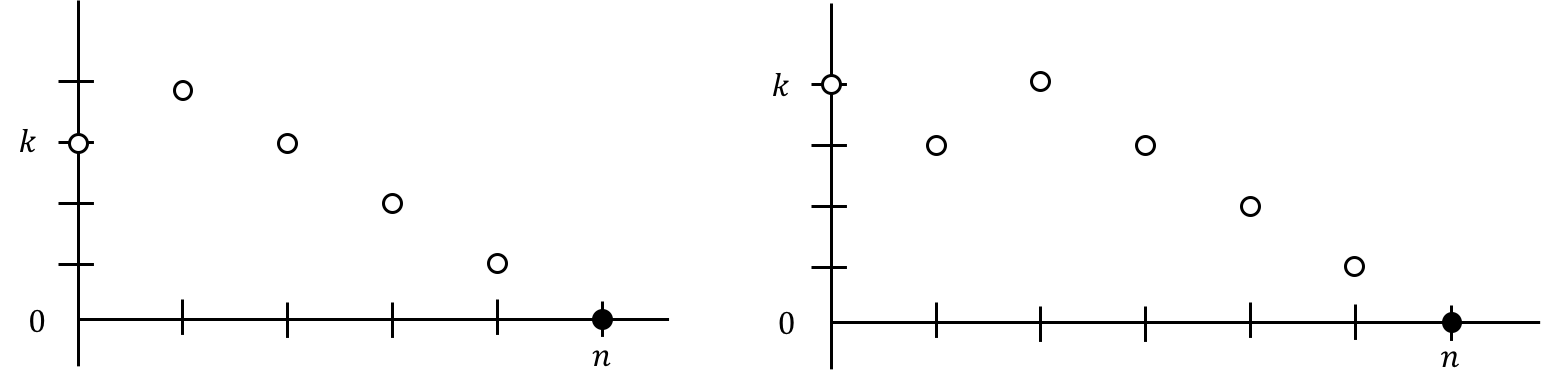
\includegraphics[width=\textwidth]
    {figure bernoul random walk.png}}
    \caption{ Trajectoires de marches aléatoires de Bernoulli (pour visualiser $\{H_0=n | X_0=k\}$)}
  \end{figure}

On a que : $$ \mathbb{P}(H_0=n \mid X_0=k) = \frac{k}{n} {{n}\choose{(n+k)/2}} q^{(n+k)/2} p^{(n-k)/2}  \quad \quad \text{si } n+k \text{ est pair, 0 sinon.}$$

La preuve de ce résultat nous vient de [13] Grimmett-Stirzaker (2001, (15), page 79), et nous allons en donner une intuition. \par 
Si $Y_n$ est notre marche aléatoire discrète de Bernoulli, on peut la formaliser de la manière suivante : $Y_0=k$ et $\forall n \in \mathbb{N}^*$, $$Y_n = k + \sum_{i=1}^n A_i, $$ où les $A_i$ sont des variables de Bernoulli i.i.d. de paramètre $p$ (\textit{i.e.} $\forall i, A_i \sim \mathcal{B}(p))$. $Y_n$ est donc la position de notre marche après $n$ étapes, en ayant commencé à $k$. L'idée est désormais d'exprimer la probabilité de l'évènement $\{H_0=n \mid X_0=k \}$ en termes de \textit{chemins}. En effet, la probabilité que les $n$ premiers pas suivent un chemin $s = (s_0, s_1, ..., s_n)$ est de $p^r q^l$, où $r$ et $l$ sont respectivement le nombre de pas vers le haut (c.-à-d. tel que $A_i=+1$) et le nombre de pas vers le bas (c.-à-d. $A_i=-1$).\par 
Ainsi, on a : $$\mathbb{P}(X_n=0 \mid X_0=k) = \sum_r M_n^r(k,0) p^r q^{n-r}, \quad \quad \quad (1.1) $$ où $M_n^r(k,0)$ est le nombre de chemins $s = (s_0, s_1, ..., s_n)$ tels que $s_0=k$ et $s_n=0$. Il s'agit donc de déterminer la valeur de $M_n^r(k,0)$.\par 

On a $r+l=n$ (c.-à-d. que le nombre de pas vers le bas et vers le haut vaut le nombre de pas totaux) et $r-l = 0-k \Leftrightarrow l-r=k$ (c.-à-d. que la différence entre le nombre de pas vers le haut et vers le bas    vaut la différence de valeur finale). Ainsi, $r=(n+k)/2$ et $l=(n-k)/2$. On peut donc réinjecter dans (1.1) et on obtient : $$\mathbb{P}(X_n=0 \mid X_0=k) = {{n}\choose{(n+k)/2}} p^{(n+k)/2} q^{(n-k)/2} \quad \quad \text{si } n+k \text{ est pair, 0 sinon.} $$

A travers ce calcul, on obtient la probabilité que notre marche soit égale à 0 au temps $n$. Mais ce que nous étudions ici, c'est la probabilité que notre marche soit égale à 0 au temps $n$ \textit{pour la première fois}. Il faut donc rajouter une condition : on s'intéresse désormais à $P(X_n=0 \mid X_1X_2...X_{n-1} \neq 0)$. Cela nous amène à compter le nombre de chemins qui passent par 0 avant le temps $n$. Le théorème du ballottage nous dit que $k/n$ chemin ne passent jamais par 0 avant le temps $n$, d'où l'on obtient finalement que : 
$$ \mathbb{P}(H_0=n \mid X_0=k) = \frac{k}{n} {{n}\choose{(n+k)/2}} q^{(n+k)/2} p^{(n-k)/2}  \quad \quad \text{si } n+k \text{ est pair, 0 sinon.}$$\par 

On a par ailleurs, d'après [13] Grimmett- Stirzaker (2001, Chapter 6), que $J_n \sim \Gamma(c,n)$, donc $\forall t \in \mathbb{R}^{+*}$, $$ 
F_{J_n}(t) = \mathbb{P}(J_n < t) = \int_0^t \frac{c^n}{(n-1)!} e^{-cu} u^{n-1} du $$ avec $\Gamma(n) = (n-1)!$ car $n$ est entier. \par

Si maintenant on décompose l'évènement $\{X_t=0\}$ avec les différentes "briques élémentaires" que nous venons de construire, on a : 
$$ \{X_t=0\} = \bigcup\limits_{n \in \mathbb{N}} \{H_0=n \mid X_0=k\} \cap \{J_n \leq t\}, $$ en se rappelant que $H_0$ est le plus petit temps où $(X_{J_n})_{n \geq 0}$ touche $0$. 

En effet, l'évènement $\{X_t=0\}$ revient à savoir, pour chaque $n$, si $H_0$ vaut $n$ (sachant un nombre d'espèce de départ $k$ fixé), et que le temps discret $J_n$ associé est inférieur à $t$. Et on peut restreindre l'union entre $n=k$ et l'infini car il est impossible que $H_0$ soit égal à $n$ si $n<k$ (car la marche de Bernoulli démarre à $k$ et met donc au moins $k$ étapes à atteindre $0$). 

Ainsi, \begin{eqnarray*}
    \mathbb{P}(X_t=0) & = & \mathbb{P}(\bigcup\limits_{n=k}^{+\infty} \{H_0=n \mid X_0=k\} \cap \{J_n \leq t\}) \\
    & = & \int_0^t \sum_{n=k}^{+\infty} \frac{c^n}{(n-1)!} e^{-cu} u^{n-1} P(H_0=n|X_0=k) du \\
    & = & \int_0^t e^{-cu} \frac{k}{u} (\frac{q}{p})^{k/2} I_k(2cu \sqrt{pq}).
\end{eqnarray*}

La simplification du calcul précédent est directe dès lors que l'on réinjecte $\mathbb{P}(H_0=n \mid X_0=k)$ et que l'on remplace $p$ et $q$ par leurs valeurs correspondantes $\mu$ et $\lambda_f$. Cela conclut la deuxième partie de la preuve, autour de ce résultat central : $\forall t \in \mathbb{R}^+$, 

$$ \boxed{\mathbb{P}(\tau_f^k>t)=1-(\frac{\mu}{\lambda_f})^{k/2} \int_0^t e^{-(\mu+\lambda_f)u} \frac{k}{u} I_k(2\sqrt{\mu\lambda_f}u) du} $$

\subsection{Comportement asymptotique du temps de survie}

\subsubsection{Dans le cas sous-critique (\texorpdfstring{$\lambda_f < \mu$}{}) (2.5.a.)}

On va maintenant s'intéresser à la troisième partie de la preuve, celle qui concerne la caractérisation du comportement à long terme de la variable $\tau_f^k$. \par 

On commence par encadrer $I_k(x)$ pour $k$ fixé dans $\mathbb{N}^*$ et $x$ suffisamment grand. D'après Abramowitz et Stegun (1992, page 377, équation 9.7.1) [14], on a : 
$$ I_k(x) \approx \frac{e^x}{\sqrt{2\pi x}} (1 - \frac{4k^2-1}{8x} + \frac{(4k^2-1)(4k^2-9)}{2! (8x)^2} - ...), $$
ce qui donne l'encadrement suivant : 
\begin{equation}
    \frac{e^x}{\sqrt{2\pi x}} (1 - \frac{4k^2 -1}{8x}) \leq I_k(x) \leq  \frac{e^x}{\sqrt{2\pi x}}.
\end{equation}


La preuve de cet encadrement fait appel à la théorie sur les fonctions de Bessel et dépasse très largement la portée de ce TER. 
On utilise cette inégalité avec $x=2\sqrt{\mu \lambda_f}u$ (qui est donc directement proportionnel à $u$, on voudra donc $u$ suffisamment grand, et non pas $x$ suffisamment grand, comme écrit dans l'article), et on multiplie partout par le facteur $\frac{e^{-(\mu+\lambda_f)u}}{u}$. On obtient d'une part :

$$ \frac{e^{\sqrt{\mu \lambda_f}u}}{2\sqrt{\pi}\sqrt{u}(\mu \lambda_f)^{1/4}} \times \frac{e^{-(\mu+\lambda_f)u}}{u} (1 - \frac{4k^2-1}{16\sqrt{\mu \lambda_f}u}) \leq \frac{e^{-(\mu+\lambda_f)u}}{u} \times I_k(2\sqrt{\mu \lambda_f}u) $$

et d'autre part : 

$$ \frac{e^{-(\mu+\lambda_f)u}}{u} \times I_k(2\sqrt{\mu \lambda_f}u) \leq \frac{e^{\sqrt{\mu \lambda_f}u}}{2\sqrt{\pi}\sqrt{u}(\mu \lambda_f)^{1/4}} \times \frac{e^{-(\mu+\lambda_f)u}}{u} $$

Ce qui équivaut à : 

$$ \frac{1}{2\sqrt{\pi}(\mu \lambda_f)^{1/4}} \times \frac{e^{-(\sqrt{\mu}-\sqrt{\lambda_f})^2 u}}{u^{3/2}} (1 - \frac{4k^2-1}{16\sqrt{\mu \lambda_f}u}) \leq \frac{e^{-(\mu+\lambda_f)u}}{u} \times I_k(2\sqrt{\mu \lambda_f}u) $$

et 

\begin{equation}
    \frac{e^{-(\mu+\lambda_f)u}}{u} \times I_k(2\sqrt{\mu \lambda_f}u) \leq \frac{1}{2\sqrt{\pi}(\mu \lambda_f)^{1/4}} \times \frac{e^{-(\sqrt{\mu}-\sqrt{\lambda_f})^2 u}}{u^{3/2}}
\end{equation}


Posons alors $\gamma = (\sqrt{\mu} - \sqrt{\lambda_f})^2$. L'article dit que l'on "observe" que : 
\begin{equation}
    (\frac{1}{\gamma}\frac{1}{t^{3/2}}-\frac{4k^2-1}{2\gamma^2}\frac{1}{t{^5/2}}) e^{-\gamma t} \leq \int_t^{+\infty}\frac{e^{-\gamma u}}{u^{3/2}} du \leq \frac{1}{\gamma}\frac{1}{t^{3/2}}.
\end{equation}

Plus précisément, cette inégalité est issue d'une intégration par parties (IPP) de l'intégrale centrale, IPP que l'on va détailler ci-dessous.

\textbf{Partie droite de l'inégalité (3).} On rappelle que, si $u$ et $v$ sont des fonctions de classe $\mathcal{C}^1$ sur un intervalle $I \subset \mathbb{R}\cup \{\pm \infty\}$, et sous réserve de convergence,

$$ \int_J u(x) v'(x) dx = [uv]_J - \int_J u'(x)v(x) dx, \quad \text{ avec } J \subset I$$

Ici, si l'on pose, 
$$ \left\{
    \begin{array}{ll}
      u(x) = x^{3/2} & \Rightarrow \quad u'(x) = \frac{3}{2} x^{-5/2} \\
      v'(x) = e^{-\gamma x}& \Leftarrow \quad v(x) = -\frac{1}{\gamma} e^{-\gamma x}
    \end{array}
  \right.$$

on a :

\begin{eqnarray*}
    \int_t^{+\infty} \frac{e^{-\gamma x}}{x^{3/2}} dx & = & \left[ - \frac{1}{\gamma} x^{-3/2} e^{-\gamma x}\right]_t^{+\infty} - \int_t^{+\infty} \frac{1}{\gamma} \frac{3}{2} x^{-5/2} e^{-\gamma x} dx \\
    & = & t^{-3/2} \frac{e^{-\gamma t}}{\gamma} - \int_t^{+\infty} \frac{1}{\gamma} \frac{3}{2} x^{-5/2} e^{-\gamma x} dx \\
    & \leq & \frac{1}{\gamma} \frac{e^{-\gamma t}}{t^{3/2}} 
\end{eqnarray*}

car $x \mapsto \frac{1}{\gamma} \frac{3}{2} x^{-5/2} e^{-\gamma x}$ est positive sur $\mathbb{R}^{+*}$, donc l'intégrale de cette fonction entre $t$ et $+\infty$ est positive. Toutes les fonctions sont bien de classe $\mathcal{C}^1$ et toutes les intégrales considérées sont convergentes, ce dont on peut se convaincre simplement à l'aide des critères de comparaison des intégrales. Cela donne la partie droite de l'inégalité (3).

\textbf{Partie gauche de l'inégalité (3).} Ensuite, si l'on reprend l'équation ci-dessus, et que l'on applique de nouveau une IPP à $\int_t^{+\infty} \frac{3}{2\gamma} x^{-5/2} e^{-\gamma x} dx$, on obtient : 

\begin{eqnarray*}
    \int_t^{+\infty} \frac{3}{2 \gamma} x^{-5/2} e^{-\gamma x} dx & = & \left[ - \frac{3}{2\gamma^2} x^{-5/2} e^{-\gamma x}\right]_t^{+\infty} - \int_t^{+\infty} \frac{1}{\gamma} \frac{3}{2}\frac{7}{2} x^{-7/2} e^{-\gamma x} dx \\
    & = & t^{-5/2} \frac{3e^{-\gamma t}}{2\gamma^2} - \int_t^{+\infty} \frac{21}{4\gamma} x^{-7/2} e^{-\gamma x} dx \\
    & \leq & \frac{3}{2\gamma^2} \frac{e^{-\gamma t}}{t^{5/2}} \\
    & \leq & \frac{4k^2 - 1}{2\gamma^2} \frac{e^{-\gamma t}}{t^{5/2}}
\end{eqnarray*}

pour les mêmes raisons que précédemment (et parce que $ \forall k \in \mathbb{N}^*, 4k^2-1 \geq 3 $). Et ainsi, si l'on réinjecte ce résultat dans l'équation précédente, on obtient bien l'égalité (3). 

Cette inégalité nous permet d'obtenir naturellement l'équivalence suivante : $$ \boxed{\int_t^{+\infty} \frac{e^{-\gamma u}}{u^{3/2}} du \sim_{+\infty} \frac{1}{\gamma} \frac{e^{-\gamma t}}{t^{3/2}}} $$

ce qui nous donne une estimation asymptotique de l'intégrale de la \textbf{borne supérieure} de (2).

En utilisant la même IPP (c.-à-d. que l'on dérive l'exponentielle et que l'on "garde" la puissance) et en notant $\alpha = (4k^2-1)/(16\sqrt{\mu \lambda_f})$, on a encore que :
$$ \int_t^{+\infty} (1-\frac{\alpha}{u}) \frac{e^{-\gamma u}}{u^{3/2}} du \geq \int_t^{+\infty} \frac{e^{-\gamma u}}{u^{3/2}} du - \frac{\alpha}{\gamma} \frac{e^{-\gamma t}}{t^{5/2}}$$

ce qui nous donne une estimation asymptotique de l'intégrale de la \textbf{borne inférieure}  de (2). Si maintenant on réinjecte ces divers résultats dans (2), on obtient un résultat intermédiaire qui n'apparaît pas dans l'article : posons $\eta = 2\sqrt{\pi} (\mu \lambda_f)^{1/4}$ :

$$ \frac{1}{\eta} \int_t^{+\infty} \frac{e^{-\gamma u}}{u^{3/2}} ( 1 - \frac{\alpha}{u}) du \leq \int_t^{+\infty} \frac{e^{-\gamma u}}{u} I_k(2\sqrt{\mu \lambda_f} u) du \leq \frac{1}{\eta} \int_t^{+\infty}  \frac{e^{-\gamma u}}{u^{3/2}} du $$

$$ \Rightarrow \left(\frac{\mu}{\lambda_f}\right)^{k/2} \frac{k}{\eta} \int_t^{+\infty} \frac{e^{-\gamma u}}{u^{3/2}} ( 1 - \frac{\alpha}{u}) du \quad \leq \quad \mathbb{P}(\tau_f^k > t) \quad \leq \quad \left(\frac{\mu}{\lambda_f}\right)^{k/2}  \frac{k}{\eta} \int_t^{+\infty}  \frac{e^{-\gamma u}}{u^{3/2}} du $$

On n'a plus qu'à conclure en réinjectant les équivalences obtenues juste au-dessus :

$$ \boxed{\mathbb{P}(\tau_f^k > t) \sim_{+\infty} \left(\frac{\mu}{\lambda_f}\right)^{k/2} \times \frac{1}{\eta} \times \frac{k}{\gamma} \times \frac{e^{-\gamma t}}{t^{3/2}}} $$ 

Ce qui achève la preuve du corollaire (2.5.a.).

\subsubsection{Dans le cas sur-critique (\texorpdfstring{$\lambda_f > \mu$}{}) (2.5.b.)}

La preuve de (2.5.b.) est immédiate avec la remarque 2.3 : si $\lambda_f > \mu$, on a :

$$ \mathbb{P}(\tau_f^k = +\infty) = 1 - \left(\frac{\mu}{\lambda_f}\right)^k$$
et 
$$ \boxed{\mathbb{P}(t < \tau_f^k < +\infty) \sim_{+\infty} \left(\frac{\mu}{\lambda_f}\right)^{k/2} \times \frac{1}{\eta} \times \frac{k}{\gamma} \times \frac{e^{-\gamma t}}{t^{3/2}}} $$

\subsubsection{Dans le cas critique (\texorpdfstring{$\lambda_f = \mu$}{}) (2.5.c.)}

Enfin, si $\lambda_f = \mu$, on a : 

$$ \mathbb{P}(\tau_f^k > t) = \int_t^{+\infty} e^{-2\mu u}\frac{k}{u} I_k(2\mu u) du $$

$$ \Rightarrow \quad \frac{k e^{-2\mu u} e^{2\mu u}}{2 u \sqrt{\pi \mu u}} (1 - \delta_n) \leq e^{-2\mu u} \frac{k}{u} I_k(2\mu u) \leq  \frac{k e^{-2\mu u} e^{2\mu u}}{2 u \sqrt{\pi \mu u}} $$ 

$$ \Rightarrow \quad \int_t^{+\infty} \frac{k}{2\sqrt{\pi \mu}} u^{-3/2} (1 - \delta_n)du \leq \int_t^{+\infty}  e^{-2\mu u} \frac{k}{u} I_k(2\mu u) du \leq  \int_t^{+\infty}  \frac{k}{2\sqrt{\pi \mu}} u^{-3/2} du, $$ avec $\delta_n$ tel que $\delta_n \longrightarrow 0$ quand $n \rightarrow +\infty$. Or $\int u^{-3/2} du = [-2u^{-1/2}]$, 
donc $$ \int_t^{+\infty} \frac{k}{2\sqrt{\pi \mu}} u^{-3/2} du = k(\pi \mu t)^{-1/2} $$

et on obtient bien l'équivalence (2.5.c.) : 

$$ \boxed{\mathbb{P}(\tau_f^k > t) \sim_{+\infty} k (\pi \mu t)^{-1/2}} $$ 

Ce qui achève la partie consacrée aux équivalences du comportement asymptotique.

\subsection{Comparaison avec la version discrète}

Dans [6], les auteurs étudient une version du modèle relativement similaire à la notre, à ceci près qu'il s'agit d'une version discrète. Ainsi, on n'a pas un processus de Poisson mais une marche aléatoire à temps discret sur $\mathbb{N}$. 
\par 
L'objectif de l'article [6] est uniquement d'obtenir la répartition des valeurs sélectives des espèces survivantes après un temps assez long, et pas d'étudier la variable du temps de survie d'une espèce (que nous notions $\tau_f^k$). Ainsi, les auteurs se placent dans le cas où il n'y a pas d'espèce au début (c'est-à-dire $k=0$). Ensuite, à chaque temps $n$, une espèce naît avec une probabilité $p$ ou meurt avec une probabilité $1-p$. Ainsi, le nombre d'espèces vivantes au temps $n$ est une marche aléatoire sur $\mathbb{N}$ qui va à droite avec probabilité $p$ et à gauche avec probabilité $1-p$. Comme dans notre modèle, une valeur sélective est associée à chaque espèce, mais dans cet article, la valeur est choisie uniformément dans $[0,1]$ et indépendamment de toute autre chose (ce qui ne change en fait rien, cf. paragraphe de mise en contexte).
Cet article montre deux résultats importants, que l'on retrouve dans notre article principal : 

\begin{itemize}
    \item si l'on note $f_c = \frac{p}{1-p}$, le nombre d'espèces dont la valeur sélective est inférieure à $f_c$ est un processus de naissance et de mort nul récurrent, c'est-à-dire qu'il est vide infiniment souvent. 
    \item le nombre d'espèces dont la valeur sélective est comprise dans un intervalle $[a,b] \subset [f_c, 1]$ divisé par $\frac{1}{n}$ tend vers $p(b-a)$, \textit{i.e.} que la répartition des valeurs sélectives des espèces survivantes est proportionnelle à la distribution $\mathcal{U}[0,1]$. 
\end{itemize}

Ces deux résultats ressemblent fort aux résultats que nous avons obtenus dans notre article (Proposition 2.7.). En effet, dire que le nombre d'espèces dont la valeur sélective est inférieure à $f_c$ est un processus nul récurrent implique que la probabilité de survie d'une espèce de valeur sélective inférieure à $f_c$ est nulle, ce que nous avons montré avec les équivalences sur le comportement de $\tau_f^k$ à l'infini. Le deuxième résultat est similaire également, à ceci près que c'est $t$ et non plus $n$ qui tend vers l'infini, et le coefficient de proportionnalité est $\frac{\lambda}{\lambda+\mu}$ et non plus $p$. \par 

Cette proximité entre les deux modèles s'explique par le fait que notre modèle peut être discrétisé en une marché aléatoire discrète de Bernoulli qui correspond exactement à celle du modèle GMS discret, avec $p=\frac{\lambda}{\lambda+\mu}$. C'est comme cela que la preuve fonctionne : les auteurs notent les sauts $J_n$ du processus $X$, de sorte que $(X_{J_n})_{n \geq 0}$ soit un processus discret, ici une marche aléatoire de Bernoulli sur $\mathbb{N}$, ce qui permet d'aboutir à la valeur de $\mathbb{P}(\tau_f^k > t)$. Par ailleurs, il est intéressant de remarquer que l'article GMS discret [6] montre déjà que le résultat sur la distribution des valeurs sélectives des espèces survivantes est valable pour toute loi de probabilité à valeurs continues, pas seulement pour la loi uniforme sur $[0,1]$, ce que nous avons redémontré. 

\newpage

\textbf{Références} 

[1] Thomas Robert Malthus, \textit{Essai sur le principe de population}, Paris, Flammarion, 1992 \par 

[2] H.W. Watson, Problem 4001, Educational Times 26 (148),p. 115 (August 1, 1873) \par

[3] F.P.Machado, A.Roldan-Correa and R.Schinazi. "Colonization and Collapse". arXiv:1510.02704 (2015).\par

[4] R.Schinazi, "Does random dispersion help survival?" Journal of Statistical Physics, 159, (1), 101-107 (2015).\par

[5] VV Junior, FP Machado, A Roldán-Correa, "Dispersion as a survival strategy". Journal of Statistical Physics, 2016 \par

[6] H. Guiol, F. P. Machado, R. B. Schinazi, "A stochastic model of evolution". Related Fields 17 (2011), n. 2, 253-258.\par

[8] P. Bak, K. Sneppen, "Punctuated equilibrium and criticality in a simple model of evolution." Phys. Rev. Lett. 74 (1993), 4083–4086.\par

[9] C. Grejo, F.P. Machado, A. Roldn-Correa, "The fitness of the strongest individual in the subcritical GMS model." Electron. Commun. Probab. 21 (2016), n. 12, 5 pp\par

[10] S. Michael, S. Volkov, "On the generalization of the GMS evolutionary model. Markov Process. Related Fields 18 (2012), n. 2, 311-322.\par

[11] I.Ben-Ari, A.Matzavinos and A.Roitershtein. "On a species survival model." Electronic Communications in Probability, 16, 226-233. (2011).\par

[12] É. Bouchet, "Marches aléatoires en environnement aléatoire faiblement elliptique", 2014

[13] Grimmett, G. and Stirzaker, D. (2001), \textit{Probability and Random Processes}, 3rd ed. New York: Oxford Univ. Press. MR2059709 \par

[14] Abramowitz and Stegun 1992, \textit{Handbook of Mathematical Functions}, p. 377

\end{document}
